% !TEX spellcheck = en_US



% ~~~~~~~~~~~~~~~~~~~~~~~~~~~~~~~~~~~~~~~ V
% (NC) 2026 Haluk Bingol
% github.com/halukbingol/LaTeX-Templates
%
% Licensees may copy, distribute, display, and perform the work and make derivative works 
% and remixes based on it only for non-commercial purposes. 
% ~~~~~~~~~~~~~~~~~~~~~~~~~~~~~~~~~~~~~~~ A




% =====================================================================
%  Java on the Command Line -- The Concepts
%  ---------------------------------------------------------------------
%  Built on hbCisLaTeXTemplate.tex with the libraries in ../../hblib/.
%  Programs, terminal sessions and their real outputs are in codeoutput/:
%     codeoutput/<Name>.java  a program        codeoutput/<Name>.sh   a session
%     codeoutput/<Name>/      the session's project folder
%     codeoutput/<Name>.txt   what it printed, made by:  bash run_examples.sh
% =====================================================================

\documentclass[aspectratio=169,10pt,compress]{beamer}

% ~~~~~~~~~~~~~~~~~~~~~~~~~~~~~~~~~~~~~~~~~~~~~~~~~~~~~~~~~~~~~ V hblib
	\usepackage{../../hblib/hblibPresentation} % lib presentation
	\usepackage{../../hblib/hblibCodeoutput} % lib code + output
	\usepackage{../../hblib/hblibDatastructures} % lib data structures
% ~~~~~~~~~~~~~~~~~~~~~~~~~~~~~~~~~~~~~~~~~~~~~~~~~~~~~~~~~~~~~ A hblib




% xcolor, array (and the L{width} column), listings, tikz and algorithm2e come from the hblib libraries
\usepackage[T1]{fontenc}
\usepackage{lmodern}
\usepackage{booktabs}

\definecolor{gitred}{RGB}{240,80,50}
\newcommand{\win}{\textbf{Windows}}
\newcommand{\mac}{\textbf{macOS}}
%
\usetikzlibrary{fit, shapes.geometric}
\tikzset{
  file/.style={draw, thick, rounded corners=2pt, fill=blue!7, font=\ttfamily\small,
               minimum height=0.8cm, minimum width=2.2cm, align=center},
  tool/.style={font=\ttfamily\small\bfseries, text=orange!80!black},
  flow/.style={-{Stealth[length=2.5mm]}, very thick, gray!70},
  box/.style={draw, thick, rounded corners, align=center},
  lbl/.style={font=\scriptsize\sffamily, text=gray!70!black}
}



% ~~~~~~~~~~~~~~~~~~~~~~~~~~~~~~~~~~~~~~ V doc
\title[CIS111-week13- CLI]{
	CIS111-week13\\
	Java on the Command Line
}

\author[Bingol]{
	Haluk O. Bingol
}

\institute[FCIS]{
    Faculty of Computer and Information Sciences\\
    Yeditepe University
}
\date{
	{\tiny \hbTimeStamp}
}

\begin{document}
% ~~~~~~~~~~~~~~~~~~~~~~~~~~~~~~~~~~~~~~ A doc




% ~~~~~~~~~~~~~~~~~~~~~~~~~~~~~~~~~~~~~~ V frm
\begin{frame}[t,fragile]
  \titlepage
\end{frame}
% ~~~~~~~~~~~~~~~~~~~~~~~~~~~~~~~~~~~~~~ A frm




% ~~~~~~~~~~~~~~~~~~~~~~~~~~~~~~~~~~~~~~ V frm
\begin{frame}[t,fragile] \frametitle{Outline}
%  \tableofcontents[hideallsubsections]
  \begin{columns}[T]
    \begin{column}{0.48\textwidth}
      \tableofcontents[sections={1-7}, hideallsubsections]
    \end{column}
    \begin{column}{0.48\textwidth}
      \tableofcontents[sections={8-14}, hideallsubsections]
    \end{column}
  \end{columns}
\end{frame}
% ~~~~~~~~~~~~~~~~~~~~~~~~~~~~~~~~~~~~~~ A frm




% ~~~~~~~~~~~~~~~~~~~~~~~~~~~~~~~~~~~~~~ V
\hSection[Picture]{The Big Picture}{}{}
% ~~~~~~~~~~~~~~~~~~~~~~~~~~~~~~~~~~~~~~ A




% ~~~~~~~~~~~~~~~~~~~~~~~~~~~~~~~~~~~~~~ V
\subsection[Pipeline]{From source to a running program}
% ~~~~~~~~~~~~~~~~~~~~~~~~~~~~~~~~~~~~~~ A




% ~~~~~~~~~~~~~~~~~~~~~~~~~~~~~~~~~~~~~~ V frm
\begin{frame}[t,fragile] \frametitle{From source code to a running program}
  \begin{center}
  
  \begin{tikzpicture}[node distance=1.5cm]
    \node[file] (src) {Hello.java\\ \scriptsize source};
    \node[file, right=1.25cm of src] (cls) {Hello.class\\ \scriptsize bytecode};
    \node[file, right=1.25cm of cls] (jar) {hello.jar\\ \scriptsize archive};
    \node[box, fill=green!10, right=1.25cm of jar, minimum height=0.8cm, minimum width=2.2cm] (jvm)
         {\textbf{JVM}\\ \scriptsize runs bytecode};
    \draw[flow] (src) -- node[above, tool]{javac} node[below, lbl]{compile} (cls);
    \draw[flow] (cls) -- node[above, tool]{jar} node[below, lbl]{package} (jar);
    \draw[flow] (jar) -- node[above, tool]{java} node[below, lbl]{run} (jvm);
    \draw[flow, dashed] (cls.south) to[bend right=22] node[below, lbl]{or run the classes directly} (jvm.south);
    \foreach \o/\x in {Windows/-3.4, macOS/-1.5, Linux/0.4}
      \node[box, fill=gray!10, font=\scriptsize, minimum width=1.7cm] (\o) at ($(jvm.north)+(\x,1.25)$) {\o};
    \foreach \o in {Windows, macOS, Linux} \draw[thick, gray] (jvm.north) -- (\o.south);
  \end{tikzpicture}
  
  \end{center}
  \vspace{-0.2em}
  
  \begin{itemize}\small
    
    \item \textbf{Compile once}: \hCode{javac} turns Java source into \textbf{bytecode}, instructions for a virtual machine, not for a real CPU
    
    \item \textbf{Run anywhere}: every operating system has its own JVM that executes the same \hCode{.class} and \hCode{.jar} files
    
    \item The command line is where all of this happens; IDEs (Eclipse, IntelliJ, VS Code) run the same tools for you
    
  \end{itemize}
  
\end{frame}
% ~~~~~~~~~~~~~~~~~~~~~~~~~~~~~~~~~~~~~~ A frm




% ~~~~~~~~~~~~~~~~~~~~~~~~~~~~~~~~~~~~~~ V frm
\begin{frame}[t,fragile] \frametitle{The whole pipeline in six commands}
  \lstterminal[basicstyle=\ttfamily\scriptsize]{codeoutput/Pipeline.txt}

  \vspace{0.1em}
  \small
  A real session (\hCode{\$} marks what was typed). 
  The package \hCode{edu.yeditepe.hello} became the folders
  \hCode{edu/yeditepe/hello/}; 
  the JAR is a ZIP file plus a \hCode{MANIFEST.MF} that names the main class.
\end{frame}
% ~~~~~~~~~~~~~~~~~~~~~~~~~~~~~~~~~~~~~~ A frm

% ~~~~~~~~~~~~~~~~~~~~~~~~~~~~~~~~~~~~~~ V
\subsection[JDK]{JDK, JRE, JVM}
% ~~~~~~~~~~~~~~~~~~~~~~~~~~~~~~~~~~~~~~ A




% ~~~~~~~~~~~~~~~~~~~~~~~~~~~~~~~~~~~~~~ V frm
\begin{frame}[t,fragile] \frametitle{JDK, JRE and JVM}
  \begin{columns}[T]
    \begin{column}{0.5\textwidth}
    
      \begin{tikzpicture}
        \node[box, fill=blue!5, minimum width=6.6cm, minimum height=4.6cm] (jdk) at (0,0) {};
        \node[anchor=north west, font=\small\bfseries] at (jdk.north west) {\ JDK: Java Development Kit};
        \node[anchor=north west, font=\ttfamily\scriptsize, align=left, text width=6.2cm] at ($(jdk.north west)+(0.1,-0.45)$)
             {javac jar javadoc jshell javap jdeps jlink jpackage jcmd jfr keytool jarsigner \dots};
        \node[box, fill=orange!8, minimum width=6.0cm, minimum height=2.9cm] (jre) at (0,-0.65) {};
        \node[anchor=north west, font=\small\bfseries] at (jre.north west) {\ runtime (``JRE'')};
        \node[anchor=north west, font=\scriptsize, align=left, text width=5.6cm] at ($(jre.north west)+(0.1,-0.45)$)
             {\hCode{java} launcher + class library (\hCode{java.base}, \hCode{java.sql}, \dots)};
        \node[box, fill=green!12, minimum width=5.4cm, minimum height=1.3cm, align=center, font=\scriptsize] at (0,-1.35)
             {\textbf{JVM}: class loader, interpreter,\\ JIT compiler, garbage collector};
      \end{tikzpicture}
      
    \end{column}
    \begin{column}{0.46\textwidth}
    
      \begin{itemize}\small
        
        \item \textbf{JVM}: the virtual machine that executes bytecode
        
        \item \textbf{Runtime} (JRE): JVM + standard library + the \hCode{java} command; 
        enough to \emph{run}
        
        \item \textbf{JDK}: runtime + development tools; needed to \emph{compile and package}
      \end{itemize}
      
      \begin{block}{Install a JDK}
        \small 
        Students need the JDK. 
        Since Java 11 Oracle no longer ships a separate JRE; 
        some vendors still offer JRE packages, and 
        \hCode{jlink} builds a minimal runtime for one application.
      \end{block}
      
    \end{column}
  \end{columns}
\end{frame}
% ~~~~~~~~~~~~~~~~~~~~~~~~~~~~~~~~~~~~~~ A frm




% ~~~~~~~~~~~~~~~~~~~~~~~~~~~~~~~~~~~~~~ V frm
\begin{frame}[t,fragile] \frametitle{What is inside a JDK}
  \lstterminal[basicstyle=\ttfamily\scriptsize]{codeoutput/JdkTools.txt}

  \vspace{0.1em}
  \small
  This machine runs Linux with an OpenJDK 21 build from Ubuntu; 
  on Windows and macOS the same tools are in the JDK's
  \hCode{bin} folder (on Windows with \hCode{.exe}: \hCode{javac.exe}, \hCode{java.exe}, \dots).
\end{frame}
% ~~~~~~~~~~~~~~~~~~~~~~~~~~~~~~~~~~~~~~ A frm




% ~~~~~~~~~~~~~~~~~~~~~~~~~~~~~~~~~~~~~~ V frm
\begin{frame}[t,fragile] \frametitle{The main tools}
  \footnotesize
  \begin{tabular}{@{}L{0.13\textwidth}L{0.37\textwidth}L{0.44\textwidth}@{}}
    \toprule
    \textbf{Tool} & \textbf{Does} & \textbf{Typical use} \\
    \midrule
    \hCode{javac}     & compiles \hCode{.java} to \hCode{.class}       & \hCode{javac -d classes Hello.java} \\
    \hCode{java}      & starts a JVM and runs a program             & \hCode{java -cp classes Hello}, \hCode{java -jar app.jar} \\
    \hCode{jar}       & creates and lists JAR archives              & \hCode{jar --create --file app.jar -C classes .} \\
    \hCode{javadoc}   & HTML documentation from comments            & \hCode{javadoc -d docs src/*.java} \\
    \hCode{jshell}    & interactive Java (read--eval--print loop)  & trying out expressions \\
    \hCode{javap}     & disassembles \hCode{.class} files          & \hCode{javap -c Hello} \\
    \hCode{jdeps}     & which packages and modules a JAR needs      & \hCode{jdeps app.jar} \\
    \hCode{jlink}     & builds a custom, smaller runtime            & \hCode{jlink --add-modules java.base \dots} \\
    \hCode{jpackage}  & native installer (\hCode{.exe}, \hCode{.msi}, \hCode{.dmg}, \hCode{.pkg}, \dots) & shipping to end users \\
    \hCode{jcmd}, \hCode{jfr} & inspects running JVMs              & diagnostics, profiling \\
    \bottomrule
  \end{tabular}
\end{frame}
% ~~~~~~~~~~~~~~~~~~~~~~~~~~~~~~~~~~~~~~ A frm

% ~~~~~~~~~~~~~~~~~~~~~~~~~~~~~~~~~~~~~~ V
\hSection[Getting]{Getting a JDK}{}{}
% ~~~~~~~~~~~~~~~~~~~~~~~~~~~~~~~~~~~~~~ A

% ~~~~~~~~~~~~~~~~~~~~~~~~~~~~~~~~~~~~~~ V
\subsection[Distributions]{Distributions}
% ~~~~~~~~~~~~~~~~~~~~~~~~~~~~~~~~~~~~~~ A




% ~~~~~~~~~~~~~~~~~~~~~~~~~~~~~~~~~~~~~~ V frm
\begin{frame}[t,fragile] \frametitle{One source code, many distributions}
  \begin{columns}[T]
    \begin{column}{0.52\textwidth}
      \small \textbf{OpenJDK} is the open-source project that develops Java. Several vendors build, test and ship it:
      \vspace{0.3em}

      \footnotesize
      \begin{tabular}{@{}ll@{}}
        \toprule
        \textbf{Build} & \textbf{From} \\
        \midrule
        Eclipse Temurin       & Adoptium, \hCode{adoptium.net} \\
        Oracle JDK            & Oracle \\
        Oracle OpenJDK builds & \hCode{jdk.java.net} \\
        Microsoft Build of OpenJDK & Microsoft \\
        Amazon Corretto       & Amazon \\
        Azul Zulu             & Azul \\
        BellSoft Liberica     & BellSoft \\
        \bottomrule
      \end{tabular}
    \end{column}
    \begin{column}{0.44\textwidth}
      \begin{block}{They differ in}
        \small
        
        \begin{itemize}
          \item how long a version gets security updates
          \item license terms (read them for commercial use)
          \item platforms and packaging (installer, ZIP, package manager)
          \item extras, e.g.\ some bundle JavaFX
        \end{itemize}
        
      \end{block}
      \begin{block}{For this course}
        \small Any current JDK works. 
        These slides use \textbf{Eclipse Temurin}: free, with installers for Windows and macOS.
      \end{block}
    \end{column}
  \end{columns}
\end{frame}
% ~~~~~~~~~~~~~~~~~~~~~~~~~~~~~~~~~~~~~~ A frm

% ~~~~~~~~~~~~~~~~~~~~~~~~~~~~~~~~~~~~~~ V
\subsection[Versions]{Versions and LTS}
% ~~~~~~~~~~~~~~~~~~~~~~~~~~~~~~~~~~~~~~ A




% ~~~~~~~~~~~~~~~~~~~~~~~~~~~~~~~~~~~~~~ V frm
\begin{frame}[t,fragile] \frametitle{Versions and long-term support}

  \begin{center}
  \begin{tikzpicture}[x=0.62cm]
    \draw[very thick, gray!60, -{Stealth}] (0,0) -- (21.5,0);
    \foreach \v/\y in {8/2014, 11/2018, 17/2021, 21/2023, 25/2025} {
      \pgfmathsetmacro{\x}{\v - 7}
      \fill (\x,0) circle (2.5pt);
      \node[font=\scriptsize, below=3pt] at (\x,0) {\y};
    }
    \foreach \v in {8, 11, 17, 21, 25} {
      \pgfmathsetmacro{\x}{\v - 7}
      \node[box, fill=orange!20, font=\small\bfseries, minimum width=0.9cm] at (\x,0.75) {\v};
    }
    \foreach \x in {2,3,5,6,7,8,9, 11,12,13,14,15, 17} \fill[gray!50] (\x,0) circle (1.5pt);
    \node[font=\scriptsize, text=gray] at (2.5,0.75) {9, 10};
    \node[font=\scriptsize, anchor=west] at (10.3,1.35) {a feature release every 6 months (March, September)};
  \end{tikzpicture}
  \end{center}
  
  \begin{itemize}\small
    
    \item Since Java 10 (2018), a new version every \textbf{six months}; most are supported only until the next one
    
    \item Every two years (since 17: 17, 21, 25) a \textbf{long-term support} (LTS) release, \colorbox{orange!20}{shown boxed}, gets updates for years
    
    \item Use an \textbf{LTS} for courses and production: Java 21 or 25 today. 
    Examples here were run with Java 21
    
    \item \hCode{java -version} tells you what you are running; 
    \hCode{21.0.12} means version 21, update 12
    
  \end{itemize}
\end{frame}
% ~~~~~~~~~~~~~~~~~~~~~~~~~~~~~~~~~~~~~~ A frm

% ~~~~~~~~~~~~~~~~~~~~~~~~~~~~~~~~~~~~~~ V
\subsection[Install]{Installing}
% ~~~~~~~~~~~~~~~~~~~~~~~~~~~~~~~~~~~~~~ A




% ~~~~~~~~~~~~~~~~~~~~~~~~~~~~~~~~~~~~~~ V frm
\begin{frame}[t,fragile] \frametitle{Ways to install a JDK}
  \footnotesize
  \begin{tabular}{@{}L{0.15\textwidth}L{0.42\textwidth}L{0.37\textwidth}@{}}
    \toprule
                     & \textbf{Windows}                                  & \textbf{macOS} \\
    \midrule
    Installer        & \hCode{.msi} from \hCode{adoptium.net}; tick \emph{Set JAVA\_HOME} and \emph{Add to PATH}
                     & \hCode{.pkg} from \hCode{adoptium.net} (Apple silicon: \emph{aarch64}; Intel: \emph{x64}) \\
    Package manager  & \hCode{winget install EclipseAdoptium.Temurin.21.JDK} & \hCode{brew install --cask temurin@21} \\
    Archive          & unzip the \hCode{.zip}; set \hCode{PATH} yourself & unpack the \hCode{.tar.gz}; set \hCode{PATH} yourself \\
    Installed in     & \hCode{C:\textbackslash Program Files\textbackslash Eclipse Adoptium\textbackslash jdk-21\dots} & \hCode{/Library/Java/JavaVirtualMachines/} \\
    Check            & \hCode{java -version}, \hCode{where java}             & \hCode{java -version}, \hCode{/usr/libexec/java\_home -V} \\
    \bottomrule
  \end{tabular}

  \vspace{0.6em}
  \begin{alertblock}{Close and reopen the terminal after installing}
    \small A terminal reads \hCode{PATH} when it starts; one that was open during the installation still cannot find \hCode{javac}.
  \end{alertblock}
\end{frame}
% ~~~~~~~~~~~~~~~~~~~~~~~~~~~~~~~~~~~~~~ A frm

% ~~~~~~~~~~~~~~~~~~~~~~~~~~~~~~~~~~~~~~ V
\hSection[Shell]{How the Shell Finds the Tools}{}{}
% ~~~~~~~~~~~~~~~~~~~~~~~~~~~~~~~~~~~~~~ A

% ~~~~~~~~~~~~~~~~~~~~~~~~~~~~~~~~~~~~~~ V
\subsection[PATH]{The PATH variable}
% ~~~~~~~~~~~~~~~~~~~~~~~~~~~~~~~~~~~~~~ A




% ~~~~~~~~~~~~~~~~~~~~~~~~~~~~~~~~~~~~~~ V frm
\begin{frame}[t,fragile] \frametitle{How the shell finds \hCode{javac}: \hCode{PATH}}

  \begin{center}
  \begin{tikzpicture}[x=1cm, y=1cm]
    \node[box, fill=gray!10, font=\ttfamily\small] (cmd) at (0,0) {\$ javac Hello.java};
    \node[lbl, above=2pt of cmd] {you type};
    \node[font=\small, anchor=west] at (2.2,0) {the shell looks in each \hCode{PATH} folder, in order:};
    \node[box, font=\ttfamily\scriptsize, minimum width=6.2cm, anchor=west] at (2.6,-0.9) {/usr/local/bin};
    \node[font=\scriptsize, anchor=west] at (8.9,-0.9) {no \hCode{javac} here};
    \node[box, font=\ttfamily\scriptsize, minimum width=6.2cm, anchor=west] at (2.6,-1.6) {/usr/bin};
    \node[font=\scriptsize, anchor=west] at (8.9,-1.6) {no \hCode{javac} here};
    \node[box, fill=green!12, font=\ttfamily\scriptsize, minimum width=6.2cm, anchor=west] at (2.6,-2.3) {/Library/Java/JavaVirtualMachines/\dots/bin};
    \node[font=\scriptsize\bfseries, anchor=west] at (8.9,-2.3) {found: run it};
    \draw[flow] (cmd.south) |- (2.6,-2.3);
  \end{tikzpicture}
  \end{center}
  
  \begin{itemize}\small
    
    \item \hCode{PATH} is an \textbf{environment variable}: a list of folders, searched from first to last
    
    \item The first match wins, so with two JDKs installed, \textbf{order matters}
    
    \item Not found anywhere: \win\ \hCode{'javac' is not recognized \dots}, \mac\ \hCode{zsh: command not found: javac}
    
    \item \hCode{JAVA\_HOME} is another variable: the JDK folder itself. Build tools (Maven, Gradle) and IDEs use it
    
  \end{itemize}
  
\end{frame}
% ~~~~~~~~~~~~~~~~~~~~~~~~~~~~~~~~~~~~~~ A frm




% ~~~~~~~~~~~~~~~~~~~~~~~~~~~~~~~~~~~~~~ V frm
\begin{frame}[t,fragile] \frametitle{The same ideas, different syntax}
  \small
  \begin{tabular}{@{}L{0.26\textwidth}L{0.33\textwidth}L{0.33\textwidth}@{}}
    \toprule
                            & \textbf{Windows (Command Prompt)}       & \textbf{macOS (Terminal, zsh)} \\
    \midrule
    show a variable         & \hCode{echo \%JAVA\_HOME\%}           & \hCode{echo \$JAVA\_HOME} \\
    where is a command      & \hCode{where javac}                   & \hCode{which javac} \\
    folder separator        & \hCode{\textbackslash}: \hCode{src\textbackslash Hello.java} & \hCode{/}: \hCode{src/Hello.java} \\
    path list separator     & \hCode{;} \quad (\hCode{-cp classes;lib\textbackslash a.jar}) & \hCode{:} \quad (\hCode{-cp classes:lib/a.jar}) \\
    list files              & \hCode{dir}                           & \hCode{ls} \\
    current folder          & \hCode{cd}                            & \hCode{pwd} \\
    last exit code          & \hCode{echo \%ERRORLEVEL\%}           & \hCode{echo \$?} \\
    set for this session    & \hCode{set NAME=value}                & \hCode{export NAME=value} \\
    set permanently         & \emph{System Properties, Environment Variables} & a line in \hCode{\textasciitilde/.zshrc} \\
    \bottomrule
  \end{tabular}

  \vspace{0.6em}
  \hCode{java}, \hCode{javac} and \hCode{jar} accept \hCode{/} in file paths on Windows too; the \textbf{path list} separator
  (\hCode{;} versus \hCode{:}) is the difference that really matters.
\end{frame}
% ~~~~~~~~~~~~~~~~~~~~~~~~~~~~~~~~~~~~~~ A frm

% ~~~~~~~~~~~~~~~~~~~~~~~~~~~~~~~~~~~~~~ V
\hSection[Compiling]{Compiling and Running}{}{}
% ~~~~~~~~~~~~~~~~~~~~~~~~~~~~~~~~~~~~~~ A

% ~~~~~~~~~~~~~~~~~~~~~~~~~~~~~~~~~~~~~~ V
\subsection[Packages]{Packages are folders}
% ~~~~~~~~~~~~~~~~~~~~~~~~~~~~~~~~~~~~~~ A




% ~~~~~~~~~~~~~~~~~~~~~~~~~~~~~~~~~~~~~~ V frm
\begin{frame}[t,fragile] \frametitle{Packages are folders}
  \begin{columns}[T]
    \begin{column}{0.5\textwidth}


% +++++++++++++++++++++++++++++++++++++++ V lst
%: -Lst.
\begin{lstlisting}[style=codesnippet, language=Java]
package edu.yeditepe.hello;

public class Hello { ... }
\end{lstlisting}
% +++++++++++++++++++++++++++++++++++++++ A lst


      \begin{itemize}\small
        \item The \textbf{fully qualified name} is \hCode{edu.yeditepe.hello.Hello}
        \item \hCode{javac -d classes} writes the class to \hCode{classes/edu/yeditepe/hello/Hello.class}
        \item \hCode{java} takes the \textbf{class name}, not a file name:
              \hCode{java -cp classes edu.yeditepe.hello.Hello}
      \end{itemize}
    \end{column}
    \begin{column}{0.46\textwidth}
      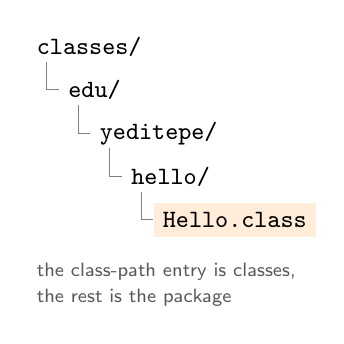
\begin{tikzpicture}[every node/.style={font=\ttfamily\small, anchor=west}, y=0.55cm]
        \node at (0,0) {classes/};
        \node at (0.4,-1) {edu/};
        \node at (0.8,-2) {yeditepe/};
        \node at (1.2,-3) {hello/};
        \node[fill=orange!15] at (1.6,-4) {Hello.class};
        \draw[gray] (0.25,-0.35) |- (0.4,-1);
        \draw[gray] (0.65,-1.35) |- (0.8,-2);
        \draw[gray] (1.05,-2.35) |- (1.2,-3);
        \draw[gray] (1.45,-3.35) |- (1.6,-4);
        \node[font=\scriptsize\sffamily, text=gray!70!black] at (0,-5.2) {the class-path entry is \hCode{classes},};
        \node[font=\scriptsize\sffamily, text=gray!70!black] at (0,-5.8) {the rest is the package};
      \end{tikzpicture}
    \end{column}
  \end{columns}
\end{frame}
% ~~~~~~~~~~~~~~~~~~~~~~~~~~~~~~~~~~~~~~ A frm

% ~~~~~~~~~~~~~~~~~~~~~~~~~~~~~~~~~~~~~~ V
\subsection[Class path]{The class path}
% ~~~~~~~~~~~~~~~~~~~~~~~~~~~~~~~~~~~~~~ A




% ~~~~~~~~~~~~~~~~~~~~~~~~~~~~~~~~~~~~~~ V frm
\begin{frame}[t,fragile] \frametitle{The class path: where \hCode{java} looks for classes}
  \begin{center}
  \begin{tikzpicture}[x=1cm, y=1cm]
    \node[box, fill=gray!10, font=\ttfamily\small] at (0,0) {\$ java -cp classes:lib/json.jar edu.yeditepe.app.Main};
    \node[box, font=\small, minimum width=2.2cm] (jdk) at (-4.2,-1.4) {the JDK's\\ own classes};
    \node[box, font=\ttfamily\small, minimum width=2.2cm] (c) at (-1.3,-1.4) {classes/};
    \node[box, font=\ttfamily\small, minimum width=2.2cm] (j) at (1.6,-1.4) {lib/json.jar};
    \node[font=\small, text=red!70!black, align=left, anchor=west] (no) at (3.3,-1.4) {not found:\\ \hCode{ClassNotFoundException}};
    \draw[flow] (jdk) -- (c);
    \draw[flow] (c) -- (j);
    \draw[flow] (j) -- (no);
    \node[lbl] at (-1.3,-2.3) {searched in this order; the first match wins};
  \end{tikzpicture}
  \end{center}
  \begin{itemize}\small
    \item The \textbf{class path} lists folders and JAR files: \hCode{-cp} (or \hCode{-classpath}, \hCode{--class-path})
    \item Default: the current folder \hCode{.} (unless the \hCode{CLASSPATH} variable is set; better leave it unset)
    \item \win\ separates entries with \hCode{;}, \mac\ (and Linux) with \hCode{:}
    \item \hCode{javac} uses a class path too, to find the classes your code uses
  \end{itemize}
\end{frame}
% ~~~~~~~~~~~~~~~~~~~~~~~~~~~~~~~~~~~~~~ A frm

% ~~~~~~~~~~~~~~~~~~~~~~~~~~~~~~~~~~~~~~ V
\subsection[Source mode]{Running a source file directly}
% ~~~~~~~~~~~~~~~~~~~~~~~~~~~~~~~~~~~~~~ A




% ~~~~~~~~~~~~~~~~~~~~~~~~~~~~~~~~~~~~~~ V frm
\begin{frame}[t,fragile] \frametitle{Running a source file directly (Java 11+)}
  \begin{columns}[T]
    \begin{column}{0.5\textwidth}
      \textbf{Classic: compile, then run}


% +++++++++++++++++++++++++++++++++++++++ V lst
%: -Lst.
\begin{lstlisting}[style=codesnippet, language=bash]
javac Hello.java      # -> Hello.class
java Hello            # run the class
\end{lstlisting}
% +++++++++++++++++++++++++++++++++++++++ A lst


      \textbf{Source-file mode}


% +++++++++++++++++++++++++++++++++++++++ V lst
%: -Lst.
\begin{lstlisting}[style=codesnippet, language=bash]
java Hello.java       # compile + run
\end{lstlisting}
% +++++++++++++++++++++++++++++++++++++++ A lst


    \end{column}
    \begin{column}{0.46\textwidth}
      \begin{itemize}\small
        \item \hCode{java Hello.java} compiles the file \textbf{in memory}; no \hCode{.class} file is written
        \item Java 11 to 21: the program must be a \textbf{single file}
        \item Java 22+: it may use other source files in the same folder tree
        \item Great for small programs and scripts; real projects still compile with \hCode{javac} and ship JARs
      \end{itemize}
    \end{column}
  \end{columns}
\end{frame}
% ~~~~~~~~~~~~~~~~~~~~~~~~~~~~~~~~~~~~~~ A frm

% ~~~~~~~~~~~~~~~~~~~~~~~~~~~~~~~~~~~~~~ V
\hSection[Packaging]{Packaging}{}{}
% ~~~~~~~~~~~~~~~~~~~~~~~~~~~~~~~~~~~~~~ A

% ~~~~~~~~~~~~~~~~~~~~~~~~~~~~~~~~~~~~~~ V
\subsection[JAR]{JAR files}
% ~~~~~~~~~~~~~~~~~~~~~~~~~~~~~~~~~~~~~~ A




% ~~~~~~~~~~~~~~~~~~~~~~~~~~~~~~~~~~~~~~ V frm
\begin{frame}[t,fragile] \frametitle{A JAR is a ZIP file with a manifest}
  \begin{columns}[T]
    \begin{column}{0.46\textwidth}
      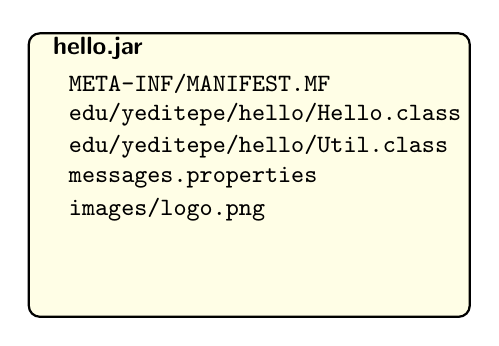
\begin{tikzpicture}[every node/.style={font=\ttfamily\small, anchor=west}, y=0.5cm]
        \node[box, fill=yellow!10, minimum width=5.6cm, minimum height=3.6cm, anchor=north west] at (-0.2,0.6) {};
        \node[font=\small\bfseries\sffamily] at (0,0.2) {hello.jar};
        \node at (0.2,-0.7) {META-INF/MANIFEST.MF};
        \node at (0.2,-1.5) {edu/yeditepe/hello/Hello.class};
        \node at (0.2,-2.3) {edu/yeditepe/hello/Util.class};
        \node at (0.2,-3.1) {messages.properties};
        \node at (0.2,-3.9) {images/logo.png};
      \end{tikzpicture}
      \vspace{0.3em}

      \small \hCode{META-INF/MANIFEST.MF}:


% +++++++++++++++++++++++++++++++++++++++ V lst
%: -Lst.
\begin{lstlisting}[style=codesnippet, language={}, basicstyle=\ttfamily\scriptsize]
Manifest-Version: 1.0
Main-Class: edu.yeditepe.hello.Hello
Class-Path: lib/json.jar
\end{lstlisting}
% +++++++++++++++++++++++++++++++++++++++ A lst


    \end{column}
    \begin{column}{0.5\textwidth}
      \begin{itemize}\small
        \item One file instead of a folder tree: classes, resources (text, images), metadata
        \item \textbf{Compressed} like a ZIP; any ZIP tool can open it
        \item \hCode{Main-Class} makes it \textbf{executable}: \hCode{java -jar hello.jar}
        \item \hCode{Class-Path} names other JARs it needs, relative to the JAR's folder
        \item A \textbf{library} JAR has no \hCode{Main-Class}; programs put it on their class path
        \item A ``fat'' (uber) JAR copies all libraries inside: one file to ship
      \end{itemize}
    \end{column}
  \end{columns}
\end{frame}
% ~~~~~~~~~~~~~~~~~~~~~~~~~~~~~~~~~~~~~~ A frm

% ~~~~~~~~~~~~~~~~~~~~~~~~~~~~~~~~~~~~~~ V
\subsection[Modules]{Modules}
% ~~~~~~~~~~~~~~~~~~~~~~~~~~~~~~~~~~~~~~ A




% ~~~~~~~~~~~~~~~~~~~~~~~~~~~~~~~~~~~~~~ V frm
\begin{frame}[t,fragile] \frametitle{Modules (Java 9+)}
  \begin{columns}[T]
    \begin{column}{0.46\textwidth}


% +++++++++++++++++++++++++++++++++++++++ V lst
%: -Lst.
\begin{lstlisting}[style=codesnippet, language=Java]
// module-info.java
module edu.yeditepe.app {
    requires edu.yeditepe.util;
    requires java.sql;
}
\end{lstlisting}
% +++++++++++++++++++++++++++++++++++++++ A lst


      \begin{center}
      \begin{tikzpicture}[mod/.style={box, fill=green!10, font=\ttfamily\scriptsize}]
        \node[mod] (a) at (0,0) {edu.yeditepe.app};
        \node[mod] (u) at (-1.6,-1.1) {edu.yeditepe.util};
        \node[mod] (s) at (1.6,-1.1) {java.sql};
        \node[mod] (b) at (0,-2.2) {java.base};
        \draw[flow] (a) -- (u); \draw[flow] (a) -- (s); \draw[flow] (u) -- (b); \draw[flow] (s) -- (b);
      \end{tikzpicture}
      \end{center}
    \end{column}
    \begin{column}{0.5\textwidth}
      \begin{itemize}\small
        \item A \textbf{module} is a named group of packages with a \hCode{module-info.java}
        \item It declares what it \textbf{requires} and which packages it \textbf{exports}; others stay hidden
        \item The JDK itself is split into about 70 modules; \hCode{java.base} is always there
        \item Modules go on the \textbf{module path} (\hCode{-p}), run with \hCode{java -p mods -m edu.yeditepe.app}
        \item Most applications still use the class path; modules matter for libraries and for \hCode{jlink}
      \end{itemize}
    \end{column}
  \end{columns}
\end{frame}
% ~~~~~~~~~~~~~~~~~~~~~~~~~~~~~~~~~~~~~~ A frm

% ~~~~~~~~~~~~~~~~~~~~~~~~~~~~~~~~~~~~~~ V
\subsection[Delivery]{Delivering an application}
% ~~~~~~~~~~~~~~~~~~~~~~~~~~~~~~~~~~~~~~ A




% ~~~~~~~~~~~~~~~~~~~~~~~~~~~~~~~~~~~~~~ V frm
\begin{frame}[t,fragile] \frametitle{Three ways to deliver a Java application}
  \begin{center}
  \begin{tikzpicture}[x=1cm, y=1cm, opt/.style={box, minimum width=4.2cm, minimum height=2.3cm, text width=3.9cm}]
    \node[opt, fill=yellow!10] at (0,0) {\textbf{1. JAR}\\[2pt]\footnotesize \hCode{app.jar}\\ user installs a JDK or JRE, then \hCode{java -jar app.jar}};
    \node[opt, fill=orange!10] at (4.8,0) {\textbf{2. Runtime image}\\[2pt]\footnotesize \hCode{jlink}: app + only the modules it needs, its own \hCode{bin/java}};
    \node[opt, fill=green!10] at (9.6,0) {\textbf{3. Native installer}\\[2pt]\footnotesize \hCode{jpackage}: \hCode{.msi}/\hCode{.exe}, \hCode{.dmg}/\hCode{.pkg}, \hCode{.deb}/\hCode{.rpm}};
    \draw[flow] (2.15,0) -- (2.65,0);
    \draw[flow] (6.95,0) -- (7.45,0);
    \node[lbl] at (4.8,-1.55) {more work for the developer, less for the user $\longrightarrow$};
  \end{tikzpicture}
  \end{center}
  \begin{itemize}\small
    \item \textbf{JAR}: smallest, one file for every OS; needs Java on the user's computer
    \item \textbf{Runtime image}: no Java installation needed; one image per OS (built on that OS)
    \item \textbf{Installer}: feels like any other app (Start menu, Applications folder); \hCode{jpackage} must run on the target OS
  \end{itemize}
\end{frame}
% ~~~~~~~~~~~~~~~~~~~~~~~~~~~~~~~~~~~~~~ A frm

% ~~~~~~~~~~~~~~~~~~~~~~~~~~~~~~~~~~~~~~ V
\hSection[Summary]{Summary}{}{}
% ~~~~~~~~~~~~~~~~~~~~~~~~~~~~~~~~~~~~~~ A

% ~~~~~~~~~~~~~~~~~~~~~~~~~~~~~~~~~~~~~~ V
\subsection[Ideas]{Big ideas}
% ~~~~~~~~~~~~~~~~~~~~~~~~~~~~~~~~~~~~~~ A




% ~~~~~~~~~~~~~~~~~~~~~~~~~~~~~~~~~~~~~~ V frm
\begin{frame}[t,fragile] \frametitle{Big ideas}
  \small
  \begin{tabular}{@{}L{0.22\textwidth}L{0.71\textwidth}@{}}
    \toprule
    \textbf{Idea} & \textbf{In one sentence} \\
    \midrule
    Bytecode        & \hCode{javac} compiles once to bytecode; any OS with a JVM runs it. \\
    JDK             & The JDK = runtime + tools; install a JDK (an LTS: 21 or 25) to develop. \\
    PATH            & The shell finds \hCode{javac} through the folders listed in \hCode{PATH}. \\
    Package         & A package is a folder tree; \hCode{java} runs a class by its full name. \\
    Class path      & \hCode{-cp} lists folders and JARs searched for classes (\hCode{;} on Windows, \hCode{:} on macOS). \\
    JAR             & A ZIP of classes and resources; \hCode{Main-Class} makes it runnable with \hCode{java -jar}. \\
    Module          & Named, encapsulated groups of packages; enable \hCode{jlink}. \\
    Delivery        & JAR, \hCode{jlink} runtime image, or \hCode{jpackage} installer. \\
    \bottomrule
  \end{tabular}
\end{frame}
% ~~~~~~~~~~~~~~~~~~~~~~~~~~~~~~~~~~~~~~ A frm




% ~~~~~~~~~~~~~~~~~~~~~~~~~~~~~~~~~~~~~~ V frm
\begin{frame}[t,fragile] \frametitle{Check yourself}
  \begin{enumerate}\small
    \item \hQuestion{Which do you need to compile Java programs: a JRE or a JDK?}
          \onslide<2->{\hRemark{A JDK: the JRE has no \hCode{javac}.}}
    \item \hQuestion{\hCode{javac -version} works, but in a new folder \hCode{java Hello} says ``Could not find or load main class''. Why?}
          \onslide<3->{\hRemark{There is no \hCode{Hello.class} on the class path (here: the current folder). Compile first or \hCode{cd}.}}
    \item \hQuestion{Where does \hCode{javac -d classes} put \hCode{package a.b; class C}?}
          \onslide<4->{\hRemark{\hCode{classes/a/b/C.class}; run it with \hCode{java -cp classes a.b.C}.}}
    \item \hQuestion{Write the class path ``folder \hCode{out} and \hCode{lib/x.jar}'' for Windows and for macOS.}
          \onslide<5->{\hRemark{\hCode{out;lib\textbackslash x.jar} and \hCode{out:lib/x.jar}.}}
    \item \hQuestion{What makes \hCode{java -jar app.jar} know which class to start?}
          \onslide<6->{\hRemark{The \hCode{Main-Class} line in \hCode{META-INF/MANIFEST.MF}.}}
    \item \hQuestion{Your users have no Java installed. Which delivery options remain?}
          \onslide<7->{\hRemark{A \hCode{jlink} runtime image or a \hCode{jpackage} installer.}}
  \end{enumerate}
\end{frame}
% ~~~~~~~~~~~~~~~~~~~~~~~~~~~~~~~~~~~~~~ A frm




% ~~~~~~~~~~~~~~~~~~~~~~~~~~~~~~~~~~~~~~ V frm
\begin{frame}[t,fragile]
	\begin{center}
		\vspace{4cm}
		\hRemark{\Huge Questions?}
	\end{center}
\end{frame}
% ~~~~~~~~~~~~~~~~~~~~~~~~~~~~~~~~~~~~~~ A frm



\end{document}
